\documentclass[11pt]{article}
\usepackage[T1]{fontenc}
\usepackage[utf8]{inputenc}
\usepackage[margin=1in]{geometry}
\usepackage{amsmath,amssymb,amsthm}
\usepackage{tikz}
\usepackage[colorlinks=true,linkcolor=blue,citecolor=blue,urlcolor=blue]{hyperref}
\hypersetup{pdfauthor={P. Graham},pdftitle={A graph whose zero-forcing polynomial is not unimodal}}
\newtheorem{theorem}{Theorem}
\newtheorem{lemma}[theorem]{Lemma}
\title{A graph whose zero-forcing polynomial is not unimodal}
\author{P. Graham\\ \small\url{https://orcid.org/0009-0007-8493-1505}}
\date{November 1, 2026}
\begin{document}
\maketitle
\begin{abstract}
The zero-forcing polynomial of a graph counts its zero-forcing sets by
cardinality. We give a graph on 73 vertices with $2096$, $1592$ and $1600$
zero-forcing sets of sizes 69, 70 and 71, respectively. This answers in the
negative the question of Boyer and coauthors whether the zero-forcing
polynomial of every graph is unimodal. The graph joins two disjoint complete
graphs, of orders 32 and 33, to four disjoint edges. The proof is a short
count: vertices in each clique have the same neighbors outside it, and a
zero-forcing set can leave at most one vertex of each clique uncolored.
Wang's Lemma 3.5 and Corollary 3.6 establish this principle more generally
and count the choices within each group by its size. We apply that
principle to this explicit graph and classify the remaining possibilities
by the numbers of uncolored vertices on each side of the join. Two
independent exact programs confirm the resulting polynomial.

This work has not yet been reviewed by experts. The proofs, the certificate checkers, the figure and the text were produced by AI models (from OpenAI and Anthropic), working under the author's direction.
\end{abstract}
\medskip
\noindent\textbf{MSC 2020:} 05C31, 05C57.\quad
\textbf{Keywords:} zero forcing, graph polynomial, unimodality.

\section{Introduction}

For a finite simple graph $H$, color an initial set $S$ blue and all other
vertices white. A blue vertex with exactly one white neighbor may color
that neighbor blue. The set $S$ is a \emph{zero-forcing set} if this rule
can color every vertex. Write $z(H;k)$ for the number of such sets of
size $k$, and
\[
 Z(H;x)=\sum_{k=0}^{|V(H)|}z(H;k)x^k.
\]
A sequence is unimodal if it is weakly increasing up to some position
and weakly decreasing thereafter. Let $\sqcup$ denote disjoint union and
$\vee$ denote graph join: the join adds every edge between its two operands.

\begin{theorem}\label{thm:main}
The graph
\[
 G=(K_{32}\sqcup K_{33})\vee(K_2\sqcup K_2\sqcup K_2\sqcup K_2)
\]
has 73 vertices and zero-forcing polynomial
\[
 Z(G;x)=x^{69}(2096+1592x+1600x^2+73x^3+x^4).
\]
In particular, the zero-forcing polynomial of a finite simple graph need
not be unimodal.
\end{theorem}

Boyer, Brimkov, English, Ferrero, Keller, Kirsch, Phillips and Reinhart
asked whether the zero-forcing polynomial of every graph is unimodal
\cite[Question 1]{boyer}. The 2019 article states this as a question;
the 2018 preprint states the affirmative assertion as Section 6,
Conjecture 1. Their Theorem 16 in that preprint proves
$z(H;i)\leq z(H;i+1)$ for $1\leq i<|V(H)|/2$.
Thus the coefficients do not decrease through the first half; the question
is whether they can decrease and then increase again later.
The decrease and subsequent increase in Theorem~\ref{thm:main} occur
beyond that range.

The six displayed cliques are modules: vertices in one clique have
identical neighbors outside it. Wang's Lemma 3.5 and Corollary 3.6 in
\cite{wang} imply that a zero-forcing set leaves at most one vertex of
each such clique uncolored. One can therefore count by choosing the
cliques containing an uncolored vertex and weighting each choice by the
product of their sizes. Wang treats the more general leaky forcing rule;
ordinary zero forcing is its case with no leaks. Section 7(3) of that
work asks about unimodality for graph classes with a bounded number of
modules of identical outside neighbors. Our graph has six such modules.
We add the explicit graph and its polynomial, whose coefficients fall and
then rise: $2096>1592<1600$. The elementary specialization is included
below, and Section 3 describes the accompanying computer checks.

The proof first excludes two uncolored vertices in one module, then counts
by how many remain on each side of the join. Choosing one on the left
contributes a factor $32+33=65$; choosing one in each left module contributes
$32\cdot33=1056$. The latter contribution occurs only at degree 71, giving
the increase from 1592 to 1600. We make no claim that 73 is the least order
of a graph with this property.

\paragraph{Related work.}
Makowsky and Rakita \cite[Conjecture 1]{makowsky} conjecture that, for
every upward monotone augmented graph property, the sequence counting the
distinguished sets of each size is unimodal for almost all graphs; their
Examples 1.10(ii) place the zero-forcing polynomial in this setting. A
single example does not bear on that question. Jacob \cite{jacob} counts, for a graph $H$ on $n$ vertices, the
sizes $i$ with $0<z(H;i)<\binom{n}{i}$, the zero forcing span, and lists
graphs for which there is exactly one such size (Proposition 13 of the
preprint); unimodality is not discussed. Menon and Singh
\cite{menon} and German \cite{german} study a different question of
\cite{boyer}, stated as \cite[Conjecture 1.1]{menon}:
$z(H;i)\leq z(P_n;i)$ for every graph $H$ on $n$ vertices and all
$i\geq1$, where $P_n$ is the path. German mentions unimodality only as a
question of \cite{boyer}. We read both preprints in full; the published
abstracts agree with them, up to two words in the first, and the
reference lists are the same. Four further papers were read only in part,
and each concerns a minimum size rather than the number of forcing sets
of each size. Brimkov, Mikesell and Hicks \cite{brimkov} compute the
zero-forcing number with satisfiability models, heuristics and polyhedral
methods, as their abstract and the survey \cite{notices} describe.
Karbasioun and Ameri's abstract \cite{fuzzy} describes bounds and an
algorithm for the zero-forcing number of fuzzy graphs. Karst, Shen,
Troxell and Vu \cite{karst} and Beaudouin-Lafon and coauthors
\cite{grids} bound the zero blocking number, the minimum size of a fort,
of Cartesian products and of grids; we read their abstracts,
introductions, section headings and references. Beaton's seminar abstract
\cite{beaton} announces conditions under which polynomials generated by
clutters are unimodal; we found no slides or paper. Cameron's list of open
problems on graph polynomials \cite{cameron}, last modified October 15,
2026, still lists unimodality of the zero-forcing polynomial as open. To
our knowledge the question was open, and the result is new as far as we
could check.

\section{Counting the forcing sets}

Call the cliques of orders 32 and 33 the \emph{left modules}, and the
four edges the \emph{right modules}. Figure~\ref{fig:graph} shows their
adjacencies. We count a zero-forcing set $S$ through its complement
$W=V(G)\setminus S$, the initially white set. A \emph{fort} is a nonempty
vertex set $F$ such that no vertex outside $F$ has exactly one neighbor
in $F$. Fast and Hicks introduced forts \cite{fast-hicks}; every
zero-forcing set meets every fort, as also stated in
\cite[Proposition 2.3]{wang}.

\begin{figure}[ht]
\centering
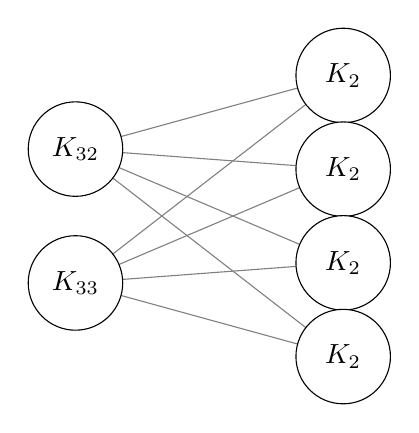
\begin{tikzpicture}[scale=.85,every node/.style={draw,circle,fill=white,minimum size=12mm}]
\coordinate (a) at (0,1); \coordinate (b) at (0,-1);
\coordinate (c) at (4,2.1); \coordinate (d) at (4,.7);
\coordinate (e) at (4,-.7); \coordinate (f) at (4,-2.1);
\foreach \l in {a,b} \foreach \r in {c,d,e,f} \draw[gray] (\l)--(\r);
\node at (a) {$K_{32}$}; \node at (b) {$K_{33}$};
\foreach \r in {c,d,e,f} \node at (\r) {$K_2$};
\end{tikzpicture}
\caption{Each circle is a clique; each line denotes all edges between
its endpoint cliques. No other intermodule edges occur.}
\label{fig:graph}
\end{figure}

\begin{lemma}[Wang {\cite[Lemma 3.5]{wang}}, specialized]\label{lem:pair}
The complement of a zero-forcing set of $G$ contains at most one vertex
from each module.
\end{lemma}
This is Wang's result with no leaks, applied to the six cliques;
the proof is included for completeness. The same twin-pair observation
appears in German's preprint \cite[Section 3, Lemma 7]{german}.
\begin{proof}
Any pair of vertices in a module is a fort: each vertex outside the pair
is adjacent either to both members or to neither. If a fort is initially
white, consider a putative first force into it. Its blue source lies
outside the fort and has a neighbor in it, hence at least two, all still
white. This contradicts the color-change rule. Thus a forcing set cannot leave
two vertices white in the same module.
\end{proof}

Every module has at least two vertices. Once the white set has at most
one vertex per module, each module therefore contains a blue vertex.
Let $r$ be the number of white vertices in the left modules and $s$ the
number in the right modules. Thus $0\leq r\leq2$ and $0\leq s\leq4$.

\begin{lemma}\label{lem:cases}
An initial set with at most one white vertex per module is forcing
exactly in the following cases:
\[
 r=0;\qquad r=1\text{ and }s<4;\qquad r=2\text{ and }s=0.
\]
\end{lemma}
\begin{proof}
If $r=0$, the blue partner of each white vertex in a right module
has that vertex as its unique white neighbor. These forces finish the
process, including the vacuous case $s=0$.

If $r=1$ and $s<4$, a completely blue right module exists. Any vertex
in that module has the unique white left vertex as its only white
neighbor and forces it. The preceding case then applies. If instead
$r=1$ and $s=4$, the blue vertex in each right module has two white
neighbors, one left and one in its own module. A blue vertex in the
left module containing the white left vertex has five white neighbors:
that vertex and the four white right vertices. A blue vertex in the
other left module has four white neighbors. There is no force, and
the initial set is not forcing.

If $r=2$ and $s=0$, a blue vertex in either left module has its own
module's white vertex as its unique white neighbor; the left modules
are not adjacent. Both white vertices can be forced. Finally, if $r=2$
and $s\geq1$, every blue vertex in a left module has $1+s\geq2$ white
neighbors, and every blue right vertex has at least the two white left
neighbors. Again no force is possible. These cases exhaust the ranges
of $r$ and $s$.
\end{proof}

\begin{proof}[Proof of Theorem~\ref{thm:main}]
For a prescribed set of modules containing white vertices, the number
of white sets is the product of their sizes. Lemma~\ref{lem:pair}
excludes every other white set. The three cases of Lemma~\ref{lem:cases}
are disjoint. If $r=0$, choosing $s$ right modules and one endpoint in
each gives $\binom4s2^s$ white sets. If $r=1$, the left choice has
$32+33=65$ possibilities, and $s$ ranges only through 3. If $r=2,s=0$,
there are $32\cdot33=1056$ white sets. Hence
\begin{align*}
 Z(G;x)
 &=\sum_{s=0}^4\binom4s2^s x^{73-s}
   +65\sum_{s=0}^3\binom4s2^s x^{72-s}+1056x^{71}\\
 &=x^{69}(2096+1592x+1600x^2+73x^3+x^4).
\end{align*}
For example, the three coefficients at the valley are
$16+65\cdot32=2096$, $32+65\cdot24=1592$, and
$24+65\cdot8+1056=1600$. All coefficients below degree 69 vanish.
Since $2096>1592<1600$, no position can be the peak of a unimodal
coefficient sequence.
\end{proof}

\section{Verification and reproducibility}

The file \texttt{data/certificate.json} lists the vertices and edges of
$G$, and two independent exact programs compute $Z(G;x)$ from it. One checks ordinary forcing on each of the 64 choices of which modules
contain a white vertex, weighted by module sizes. The other checks forcing
on all 90,882 white sets with at most one vertex per module, counting each
successful set directly. Both give the displayed polynomial, totaling
5,362 zero-forcing sets. A third check confirms that every other white set
contains a within-module pair that is a fort. Separate checks reproduce
the known polynomials of $K_6$, $P_4$ and $C_4$ and reject altered inputs.
The command \texttt{python3 -I checks/check.py} runs these checks in
seconds with standard Python; \texttt{checks/README.md} explains the inputs
and the separate checks.

\paragraph{Code and data availability.}
The certificate \texttt{data/certificate.json}, the checks in
\texttt{checks/} and this paper's source are available at
\begin{center}\footnotesize
\url{https://github.com/6/clank-lab/tree/zero-forcing-unimodality-v1/results/zero-forcing-unimodality}
\end{center}

\begin{thebibliography}{10}
\bibitem{boyer} K. Boyer, B. Brimkov, S. English, D. Ferrero, A. Keller,
R. Kirsch, M. Phillips and C. Reinhart,
\emph{The zero forcing polynomial of a graph},
Discrete Applied Mathematics 258 (2019), 35--48.
\href{https://doi.org/10.1016/j.dam.2018.11.033}{doi:10.1016/j.dam.2018.11.033}.
Preprint \href{https://arxiv.org/abs/1801.08910v1}{arXiv:1801.08910v1}, January 26, 2018.

\bibitem{wang} X. Wang,
\emph{Modular Compression of Leaky Forts and Leaky Forcing Polynomials},
Zenodo preprint, May 26, 2026.
\href{https://doi.org/10.5281/zenodo.20388397}{doi:10.5281/zenodo.20388397}.

\bibitem{fast-hicks} C. C. Fast and I. V. Hicks,
\emph{Effects of vertex degrees on the zero-forcing number and propagation
 time of a graph}, Discrete Applied Mathematics 250 (2018), 215--226.
\href{https://doi.org/10.1016/j.dam.2018.05.002}{doi:10.1016/j.dam.2018.05.002}.

\bibitem{makowsky} J. A. Makowsky and V. Rakita,
\emph{Almost unimodal and real-rooted graph polynomials},
European Journal of Combinatorics 108 (2023), 103637.
\href{https://doi.org/10.1016/j.ejc.2022.103637}{doi:10.1016/j.ejc.2022.103637}.
Preprint \href{https://arxiv.org/abs/2102.00268v4}{arXiv:2102.00268v4}, October 18, 2022.

\bibitem{jacob} B. Jacob, \emph{The zero forcing span of a graph},
in \emph{Combinatorics, Graph Theory and Computing}, Springer Proceedings
in Mathematics \& Statistics (2024), 255--267.
\href{https://doi.org/10.1007/978-3-031-52969-6_23}{doi:10.1007/978-3-031-52969-6\_23}.
Preprint \href{https://arxiv.org/abs/2309.06234v1}{arXiv:2309.06234v1}, September 12, 2023.

\bibitem{brimkov} B. Brimkov, D. Mikesell and I. V. Hicks,
\emph{Improved Computational Approaches and Heuristics for Zero Forcing},
INFORMS Journal on Computing, published online February 9, 2021.
\href{https://doi.org/10.1287/ijoc.2020.1032}{doi:10.1287/ijoc.2020.1032}.

\bibitem{notices} I. V. Hicks and B. Brimkov,
\emph{The many face(t)s of zero forcing},
Notices of the American Mathematical Society 71(2) (2024), 167--173.
\href{https://doi.org/10.1090/noti2874}{doi:10.1090/noti2874}.

\bibitem{fuzzy} A. Karbasioun and R. Ameri,
\emph{Zero forcing number of fuzzy graphs with application},
Journal of Intelligent \& Fuzzy Systems 39 (2020), 3873--3882.
\href{https://doi.org/10.3233/JIFS-192201}{doi:10.3233/JIFS-192201}.

\bibitem{karst} N. J. Karst, X. Shen, D. S. Troxell and M. Vu,
\emph{Blocking zero forcing processes in Cartesian products of graphs},
Discrete Applied Mathematics 285 (2020), 380--396.
\href{https://doi.org/10.1016/j.dam.2020.06.002}{doi:10.1016/j.dam.2020.06.002}.

\bibitem{grids} M. Beaudouin-Lafon et al.,
\emph{On the zero blocking number of rectangular, cylindrical, and M\"obius grids},
Discrete Applied Mathematics 282 (2020), 35--47.
\href{https://doi.org/10.1016/j.dam.2019.11.015}{doi:10.1016/j.dam.2019.11.015}.

\bibitem{menon} K. Menon and A. Singh,
\emph{Exploring the influence of graph operations on zero forcing sets},
Discrete Mathematics 348 (2025), 114516.
\href{https://doi.org/10.1016/j.disc.2025.114516}{doi:10.1016/j.disc.2025.114516}.
Preprint \href{https://arxiv.org/abs/2405.01423v1}{arXiv:2405.01423v1}.

\bibitem{german} S. German,
\emph{The Path-Extremal Conjecture for Zero Forcing: Distance-Hereditary
Graphs and a Split-Decomposition Reduction}, COCOON 2026,
Lecture Notes in Computer Science 16835 (2027), 409--422.
\href{https://doi.org/10.1007/978-981-92-3309-0_31}{doi:10.1007/978-981-92-3309-0\_31}.
Preprint \href{https://arxiv.org/abs/2605.10836v1}{arXiv:2605.10836v1}, May 11, 2026.

\bibitem{beaton} I. Beaton, \emph{When are Graph Polynomials Unimodal?},
University of Prince Edward Island research seminar, July 16, 2026.
\href{https://www.upei.ca/notice/2026/07/smcs-research-seminar-when-are-graph-polynomials-unimodal}{Seminar announcement and abstract}.
\bibitem{cameron} B. Cameron, \emph{Graph Polynomials} (open problems page),
University of Prince Edward Island, last modified October 15, 2026.
\href{https://www.smcs.upei.ca/~brcameron/graphpolys.html}{Problem page}.
\end{thebibliography}
\end{document}
